\documentclass{beamer}
\usetheme{metropolis}
\metroset{numbering=none,progressbar=frametitle}

\usepackage{graphicx}

\setmainfont{TeX Gyre Pagella}
\setsansfont{Montserrat}

\DeclareRobustCommand\texpage{\TeX Page}
\DeclareRobustCommand\texlive{\TeX\ Live}
\newenvironment{display}{\trivlist\item[]}{\endtrivlist}

\title{How to use \texpage}
\author{The \texpage{} Team}
\date{}

\begin{document}

\maketitle

\section{Getting Started}
\begin{frame}{Creating a \LaTeX{} Project}
  \begin{columns}
      \begin{column}{0.5\linewidth}
        \begin{itemize}
          \item Blank Project
          \item Upload Project – upload a .zip file to create a project
          \item Import from GitHub
          \item New by Template
        \end{itemize}
      \end{column}
      \begin{column}{0.5\linewidth}
        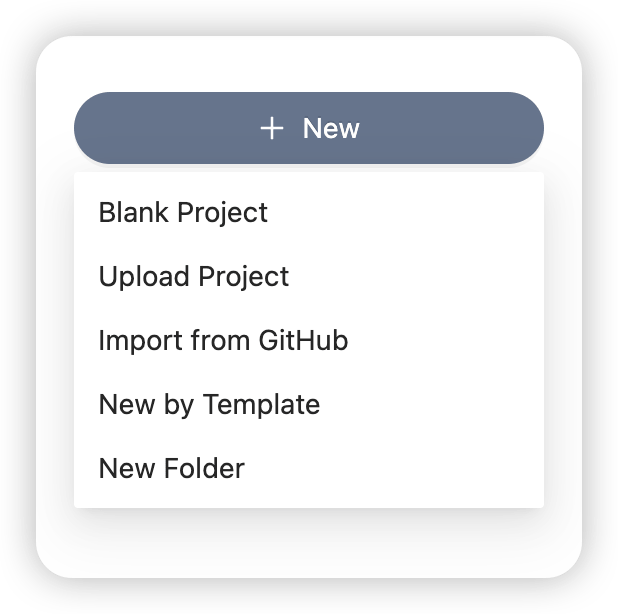
\includegraphics[width=\textwidth]{imgs/create.png}
      \end{column}
  \end{columns}
\end{frame}

\begin{frame}{Editor Layout}
  The editor consists of three resizable panels. \\
  Drag the panel borders or click the middle handles to adjust their width.
  
  \begin{display}
    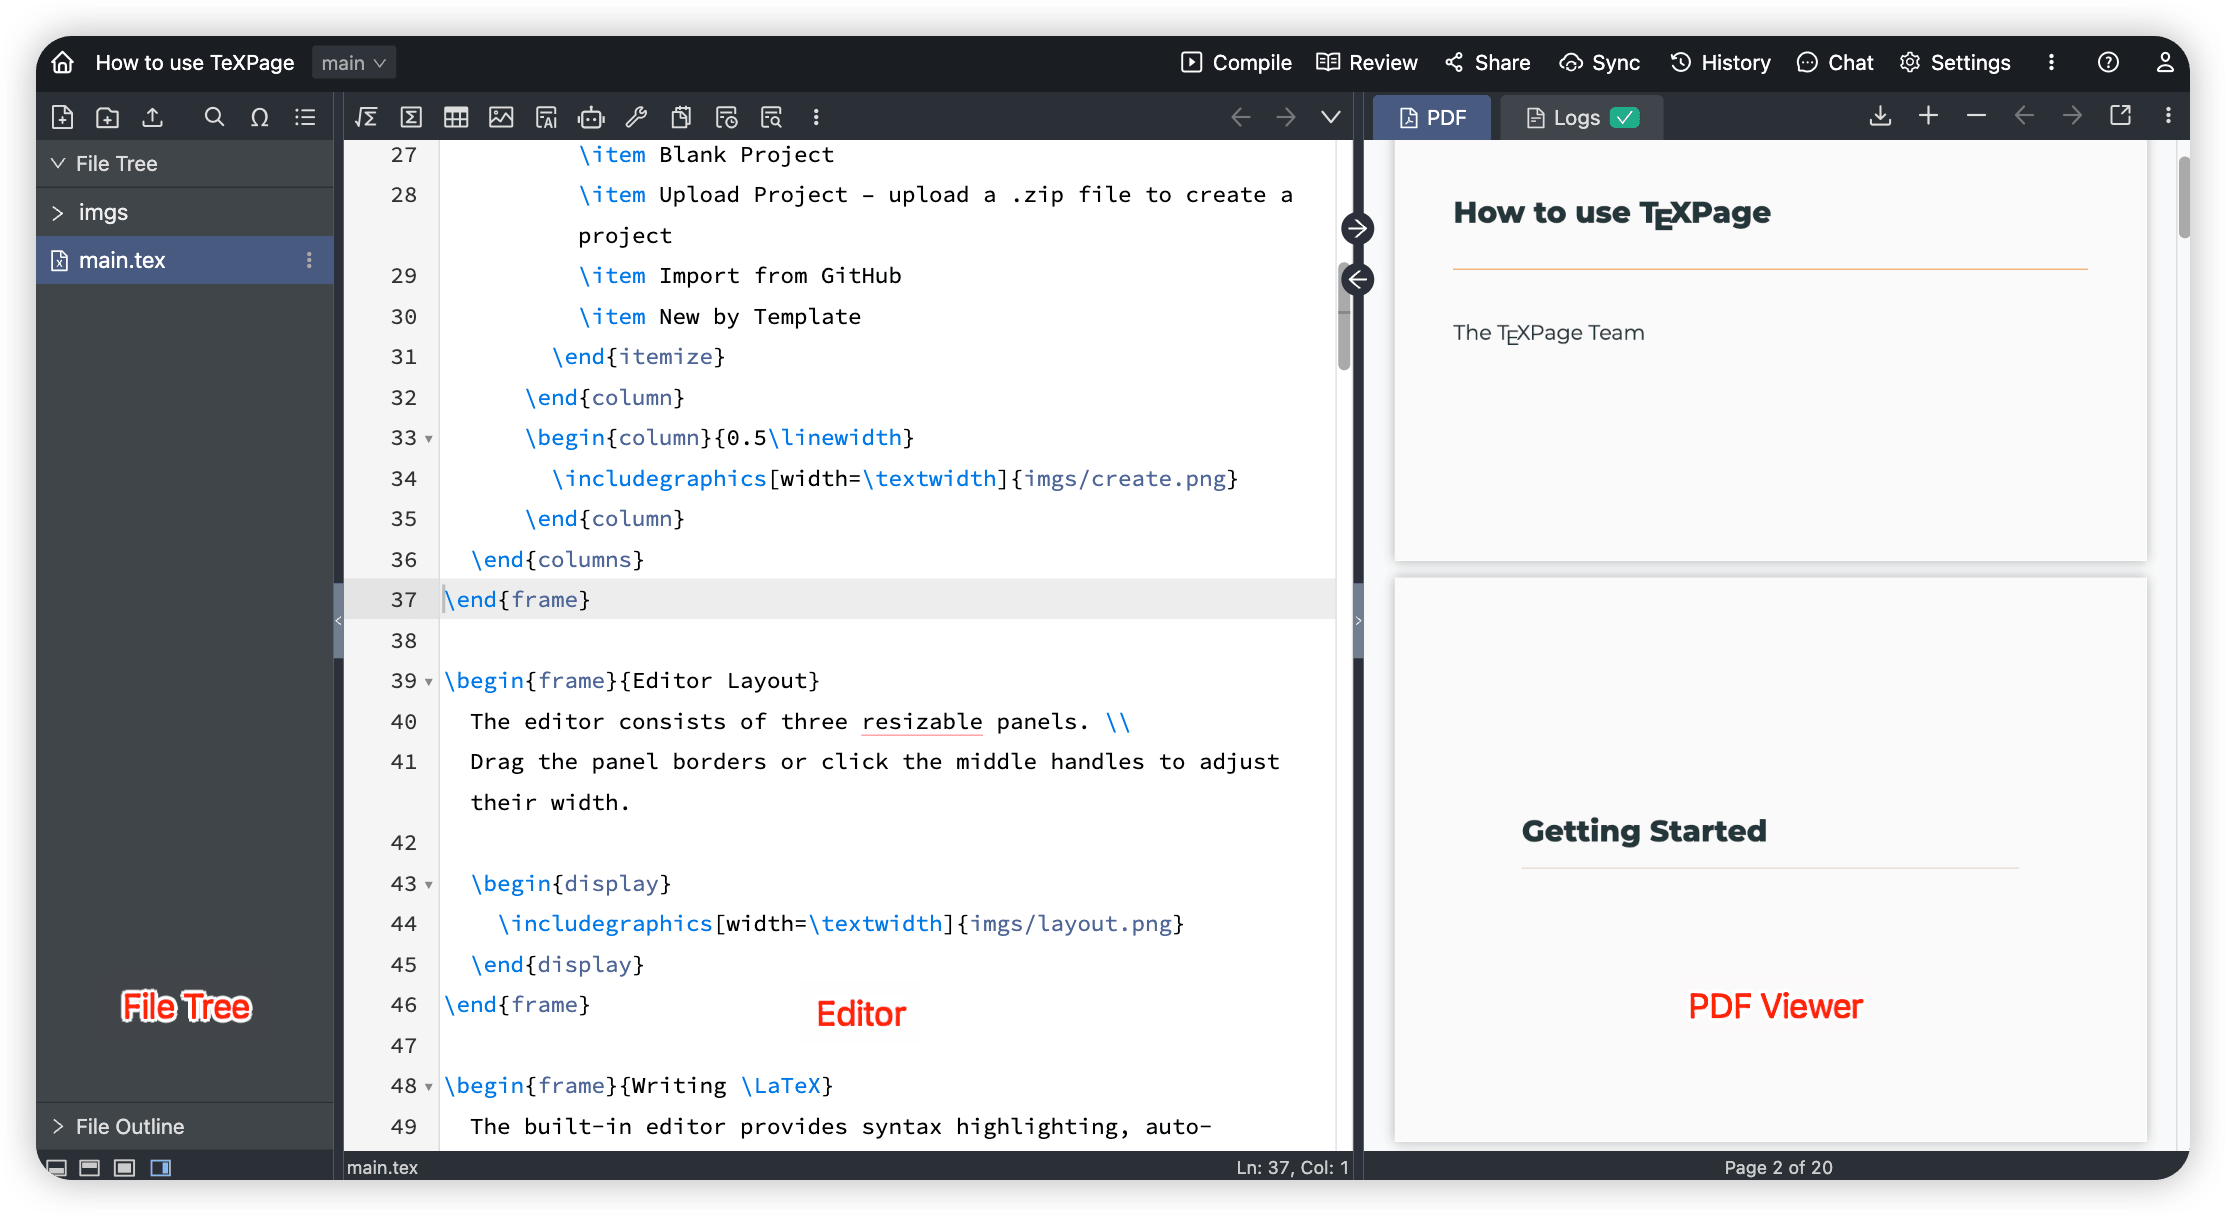
\includegraphics[width=\textwidth]{imgs/layout.png}
  \end{display}
\end{frame}

\begin{frame}{Writing \LaTeX}
  The built-in editor provides syntax highlighting, auto-completion, and other features.

  \begin{display}
    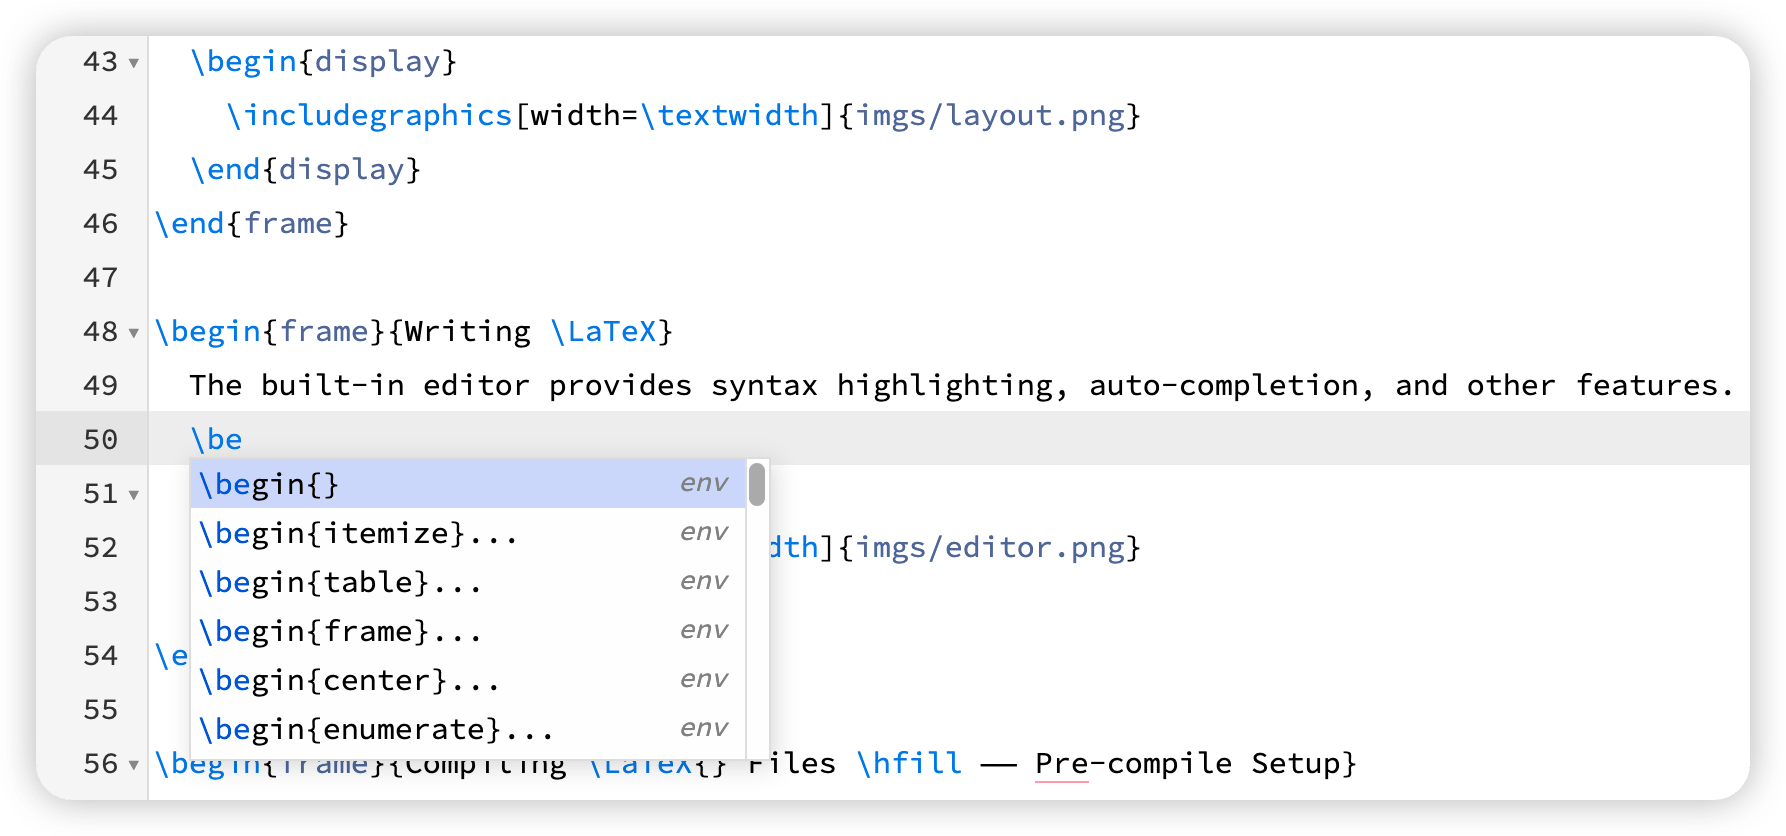
\includegraphics[width=\textwidth]{imgs/editor.png}
  \end{display}
\end{frame}

\begin{frame}{Compiling \LaTeX{} Files \hfill —— Pre-compile Setup}
  \begin{columns}
      \begin{column}{0.5\linewidth}
        \begin{itemize}
          \item Click \textbf{Settings} in the top toolbar
          \item Select the project’s main file
          \item Choose the required compiler and \texlive{} version
        \end{itemize}
      \end{column}
      \begin{column}{0.5\linewidth}
        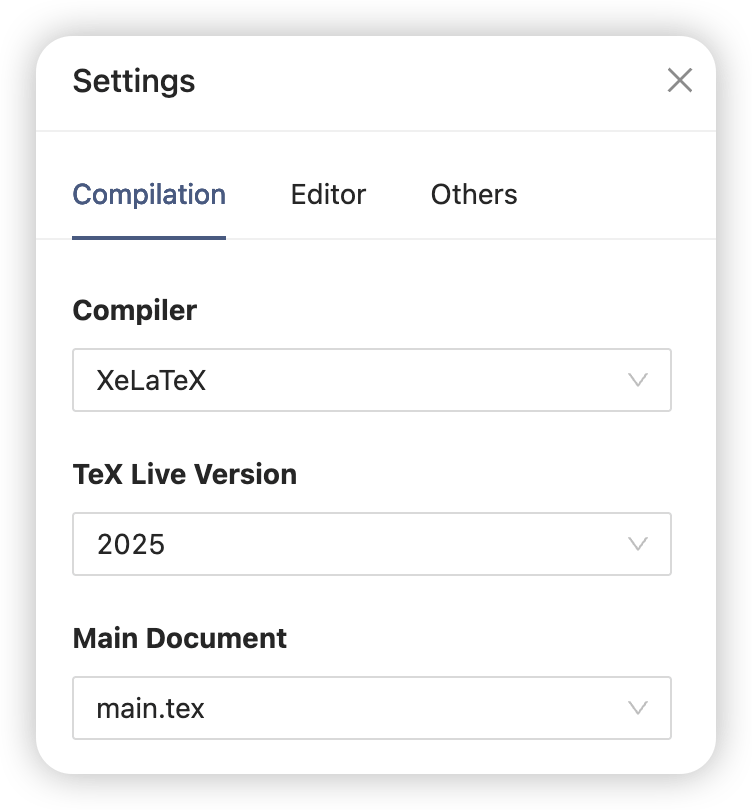
\includegraphics[width=\textwidth]{imgs/settings.png}
      \end{column}
  \end{columns}
\end{frame}

\begin{frame}{Compiling \LaTeX{} Files \hfill —— Compile}
  \begin{itemize}
    \item Click \textbf{Compile} in the top toolbar
    \item Windows: press \textbf{Ctrl + S} or \textbf{Ctrl + Enter}
    \item macOS: press \textbf{Command + S} or \textbf{Command + Enter}
  \end{itemize}
\end{frame}

\begin{frame}{Compiling \LaTeX{} Files \hfill —— PDF Preview}
  \begin{columns}
      \begin{column}{0.5\linewidth}
        \begin{itemize}
          \item Zoom in/out
          \item Navigate using PDF outline
          \item Switch between fullscreen presentation and split view
          \item Double-click a PDF element to jump to the corresponding \LaTeX{} source
        \end{itemize}
      \end{column}
      \begin{column}{0.5\linewidth}
        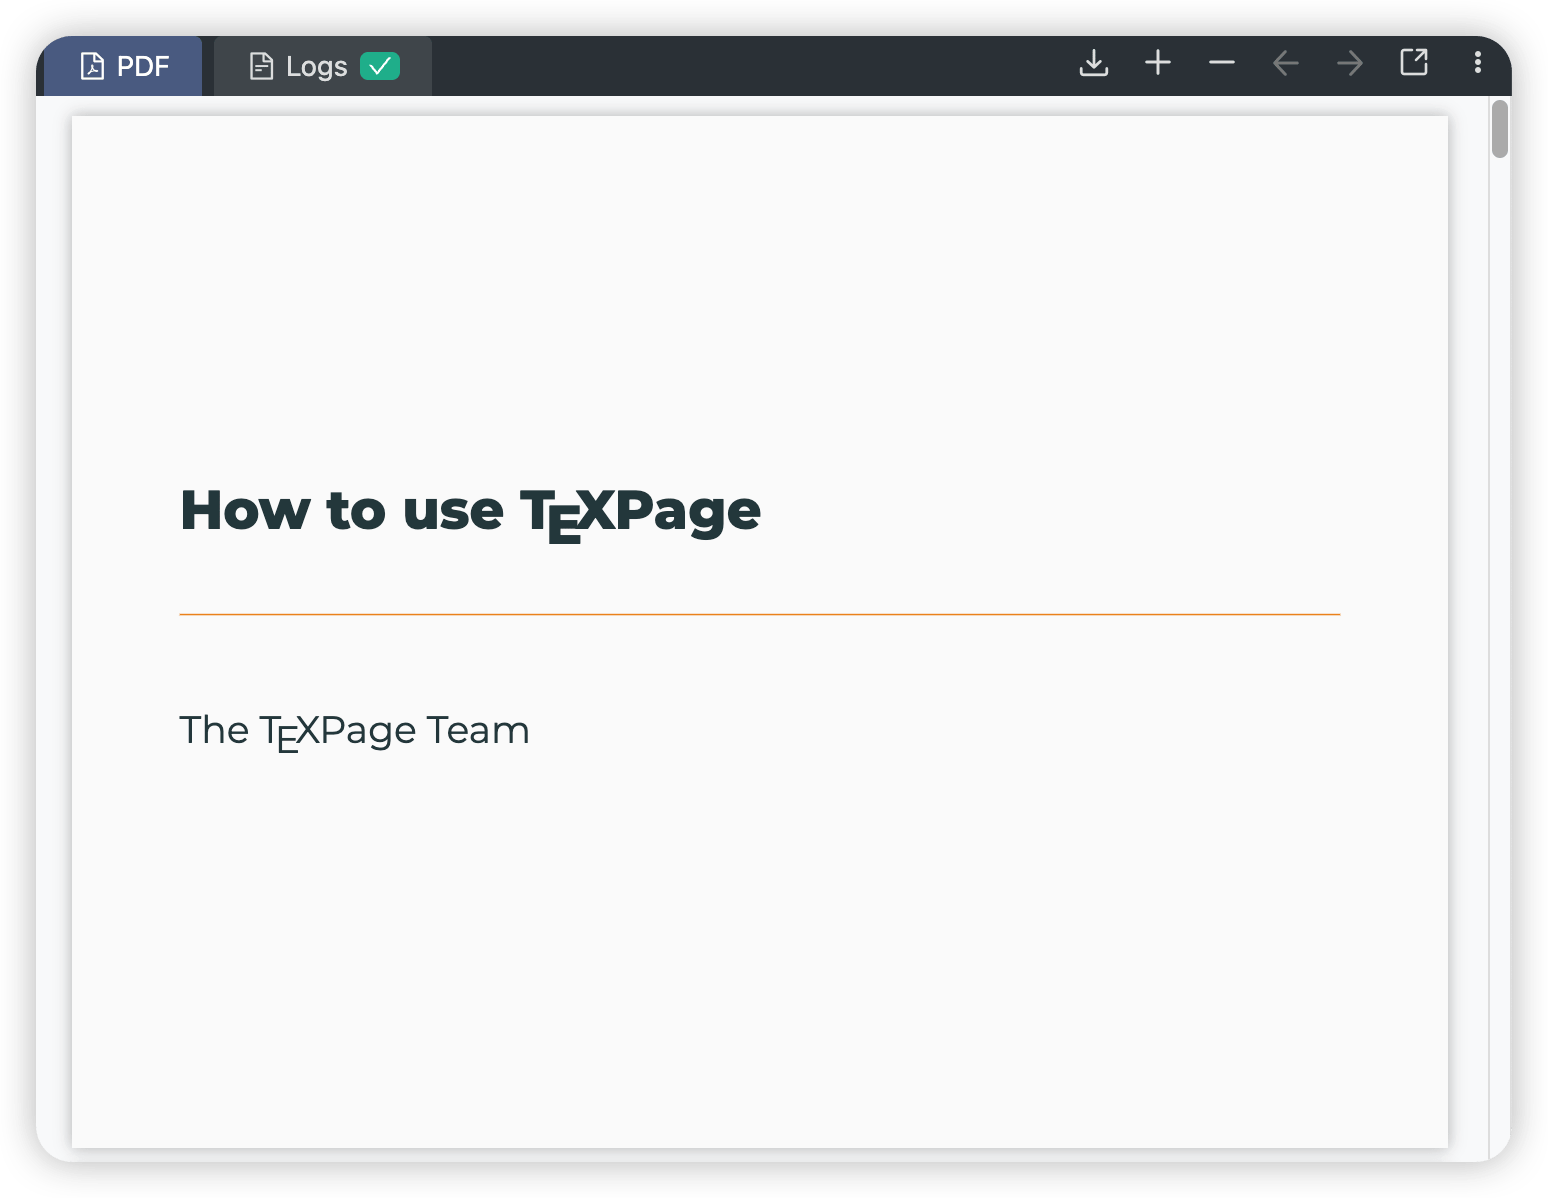
\includegraphics[width=\textwidth]{imgs/preview.png}
      \end{column}
  \end{columns}
\end{frame}

\begin{frame}{Compiling \LaTeX{} Files \hfill —— Logs}
 Compilation status is shown in the log panel above the PDF preview:
  \begin{itemize}
    \item \textbf{\color{red} Red} - Errors
    \item \textbf{\color{orange} Orange} - Warnings
    \item \textbf{\color{green!80!black}Green} Successful build (no errors/warnings)
  \end{itemize}
  To clear the build cache, click \textbf{Clear Cache} at the bottom of the log panel.
\end{frame}

\begin{frame}{Managing Project Files}
  \begin{columns}
      \begin{column}{0.5\linewidth}
        \begin{itemize}
          \item Create, rename, or delete files and folders
          \item Upload files via drag-and-drop or paste
          \item Download project files
          \item Move files by dragging them within the file tree
        \end{itemize}
      \end{column}
      \begin{column}{0.5\linewidth}
        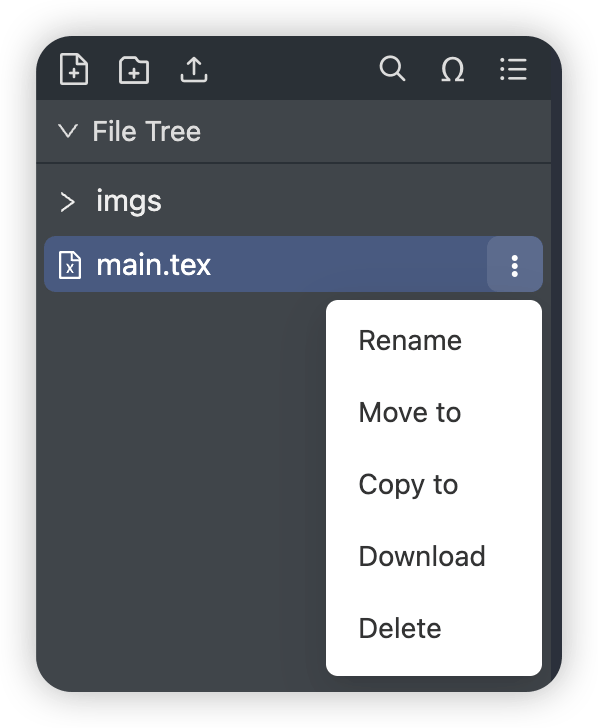
\includegraphics[width=0.9\textwidth]{imgs/fileTree.png}
      \end{column}
  \end{columns}
\end{frame}

\section{Collaboration}
\begin{frame}{Sharing Projects}
  \vspace{2ex}
  \begin{itemize}
    \item Click \textbf{Share} in the top toolbar
    \item Share via link or email
    \item Set permissions: Editor, Reviewer, Commenter, Viewer
    \item Manage collaborators directly in the sharing dialog
  \end{itemize}

  \begin{center}
    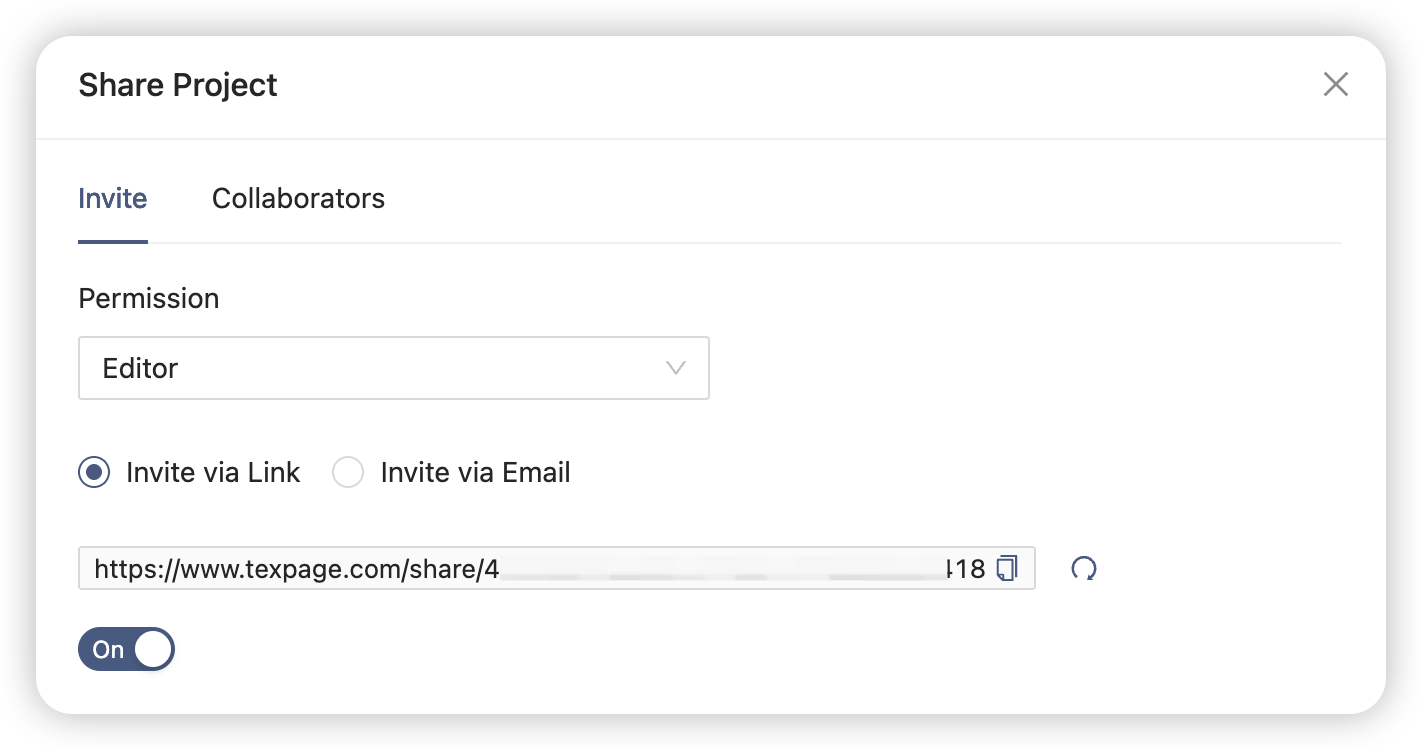
\includegraphics[width=0.8\textwidth]{imgs/share.png}
  \end{center}
\end{frame}

\begin{frame}{Review}
  \begin{columns}
      \begin{column}{0.6\linewidth}
        \begin{itemize}
          \item Comments – add or reply to comments; resolved items can be reopened
          \item Track Changes – record all edits, with options to accept or reject changes
        \end{itemize}
      \end{column}
      \begin{column}{0.4\linewidth}
        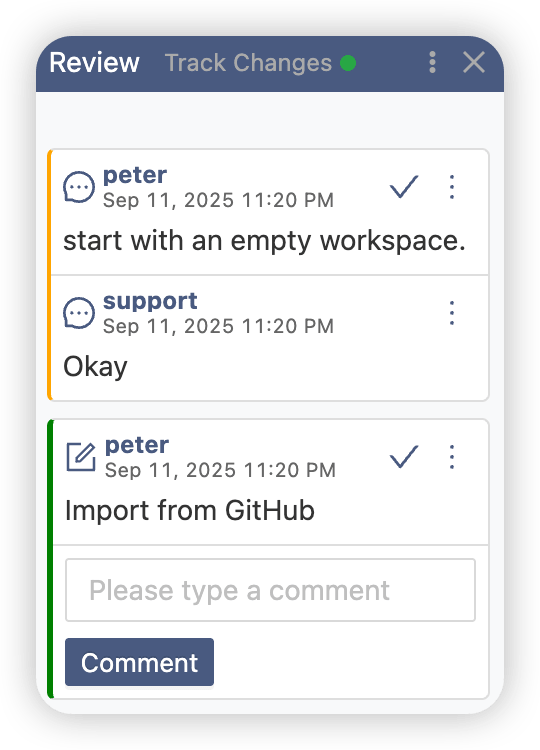
\includegraphics[width=\linewidth]{imgs/review.png}
      \end{column}
  \end{columns}
\end{frame}

\section{Version Control}
\begin{frame}{Version Control}
  \begin{columns}
      \begin{column}{0.6\linewidth}
        \begin{itemize}
          \item Default version branch is main
          \item Versions are isolated from one another
          \item Save project versions at key milestones
          \item Review data is automatically included in new versions
          \item Compare versions and export a PDF showing tracked revisions
        \end{itemize}
      \end{column}
      \begin{column}{0.4\linewidth}
        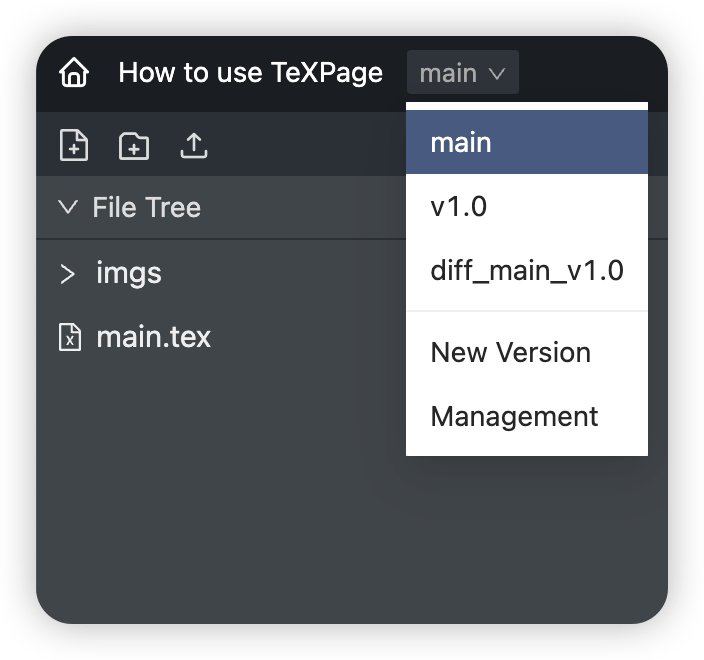
\includegraphics[width=\linewidth]{imgs/version.png}
      \end{column}
  \end{columns}
\end{frame}

\section{Built-in Tools}

\begin{frame}{Formula Editor}
  \begin{center}
    
\includegraphics[width=0.9\linewidth]{imgs/math-entry.png}
  \end{center}
  \begin{center}
    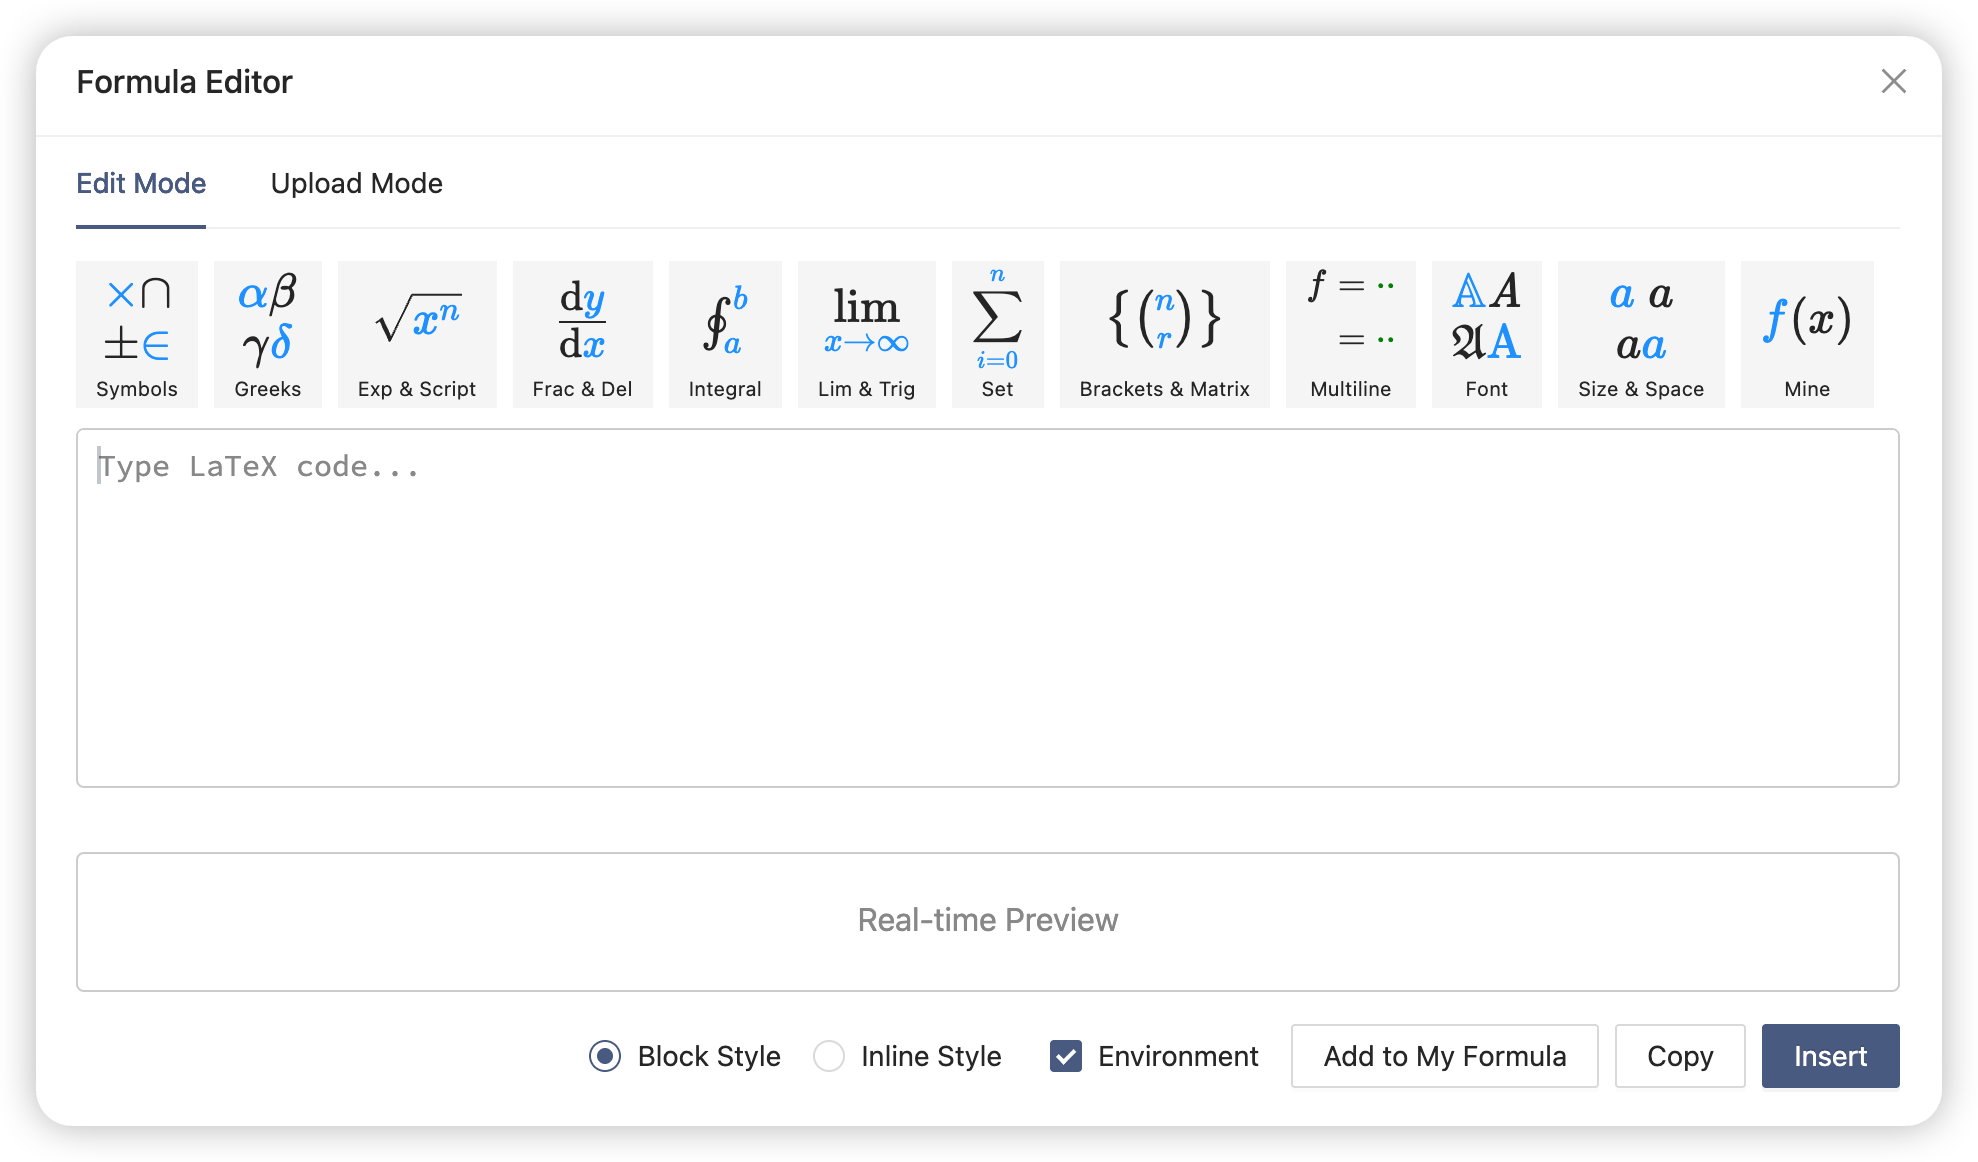
\includegraphics[width=0.9\textwidth]{imgs/math.png}
  \end{center}
\end{frame}

\begin{frame}{Table Generator}
  \begin{center}
    
\includegraphics[width=0.9\linewidth]{imgs/table-entry.png}
  \end{center}
  \begin{center}
    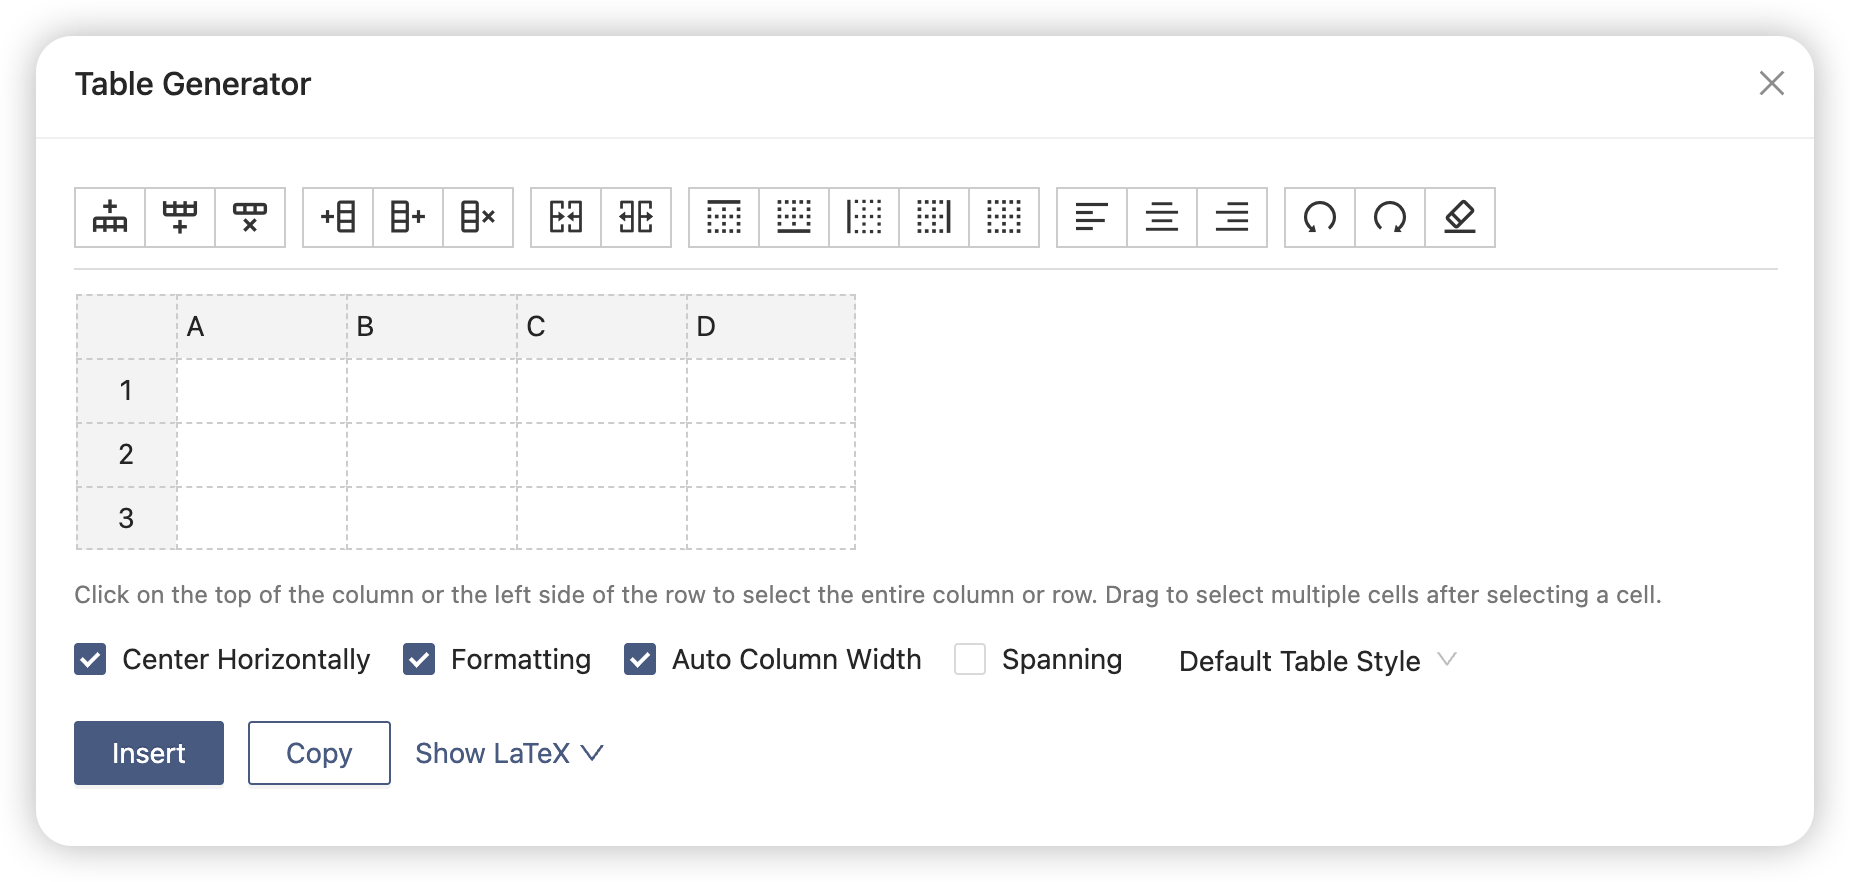
\includegraphics[width=0.9\textwidth]{imgs/table.png}
  \end{center}
\end{frame}

\begin{frame}{Figure Insertion}
  \begin{center}
    
\includegraphics[width=0.9\linewidth]{imgs/figure-entry.png}
  \end{center}
  \begin{center}
    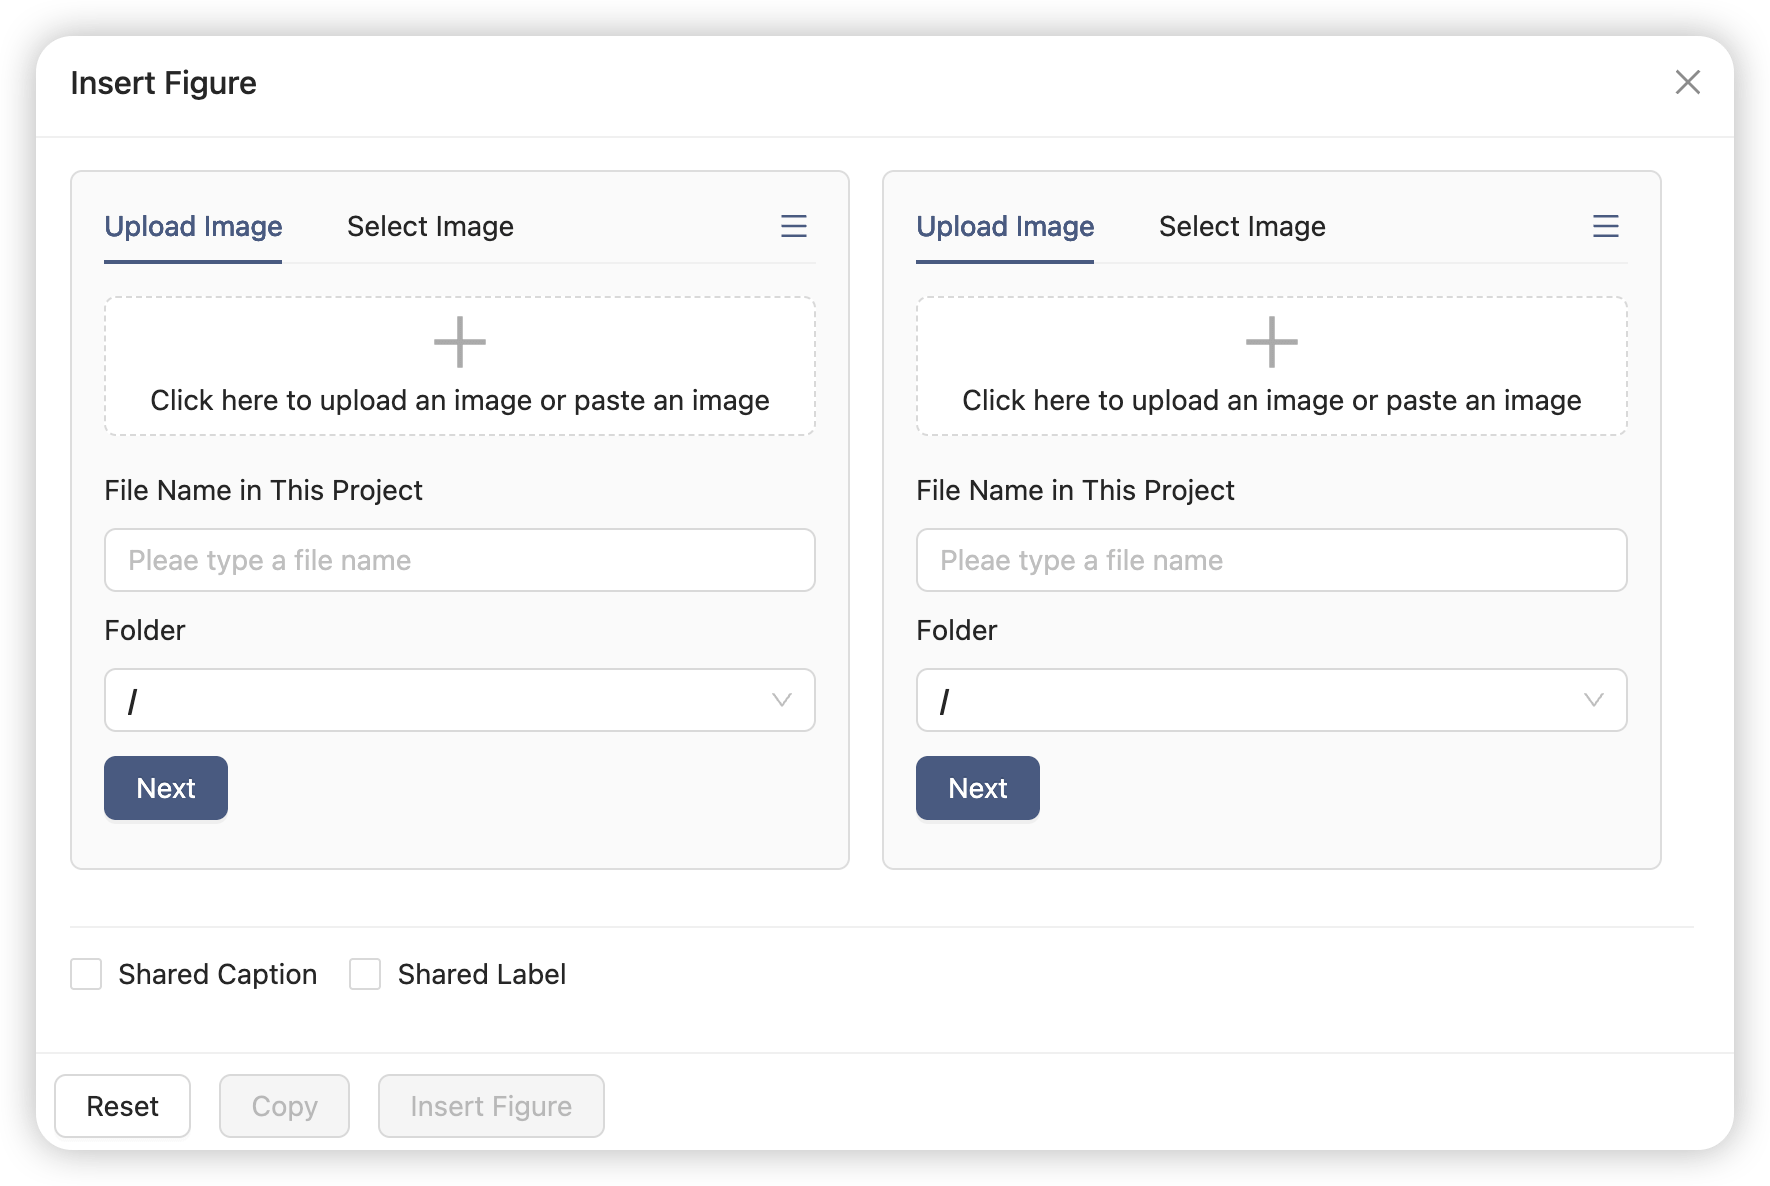
\includegraphics[width=0.9\textwidth]{imgs/figure.png}
  \end{center}
\end{frame}

\begin{frame}[standout]
  \begin{center}
    \Large Find more:
    \href{https://www.texpage.com/docs/}{\textbf{\texpage Docs{}>>}}
  \end{center}
\end{frame}

\end{document}
